\chapter{Dimensionamento de Redes Óticas Opacas e Transparentes}
\label{chapter2}

\section{Elementos de Rede}
\label{networkArchitecture}

\subsection{Arquitetura das Ligações}

\begin{figure}[H]
  \label{cisco}
  \begin{center}
    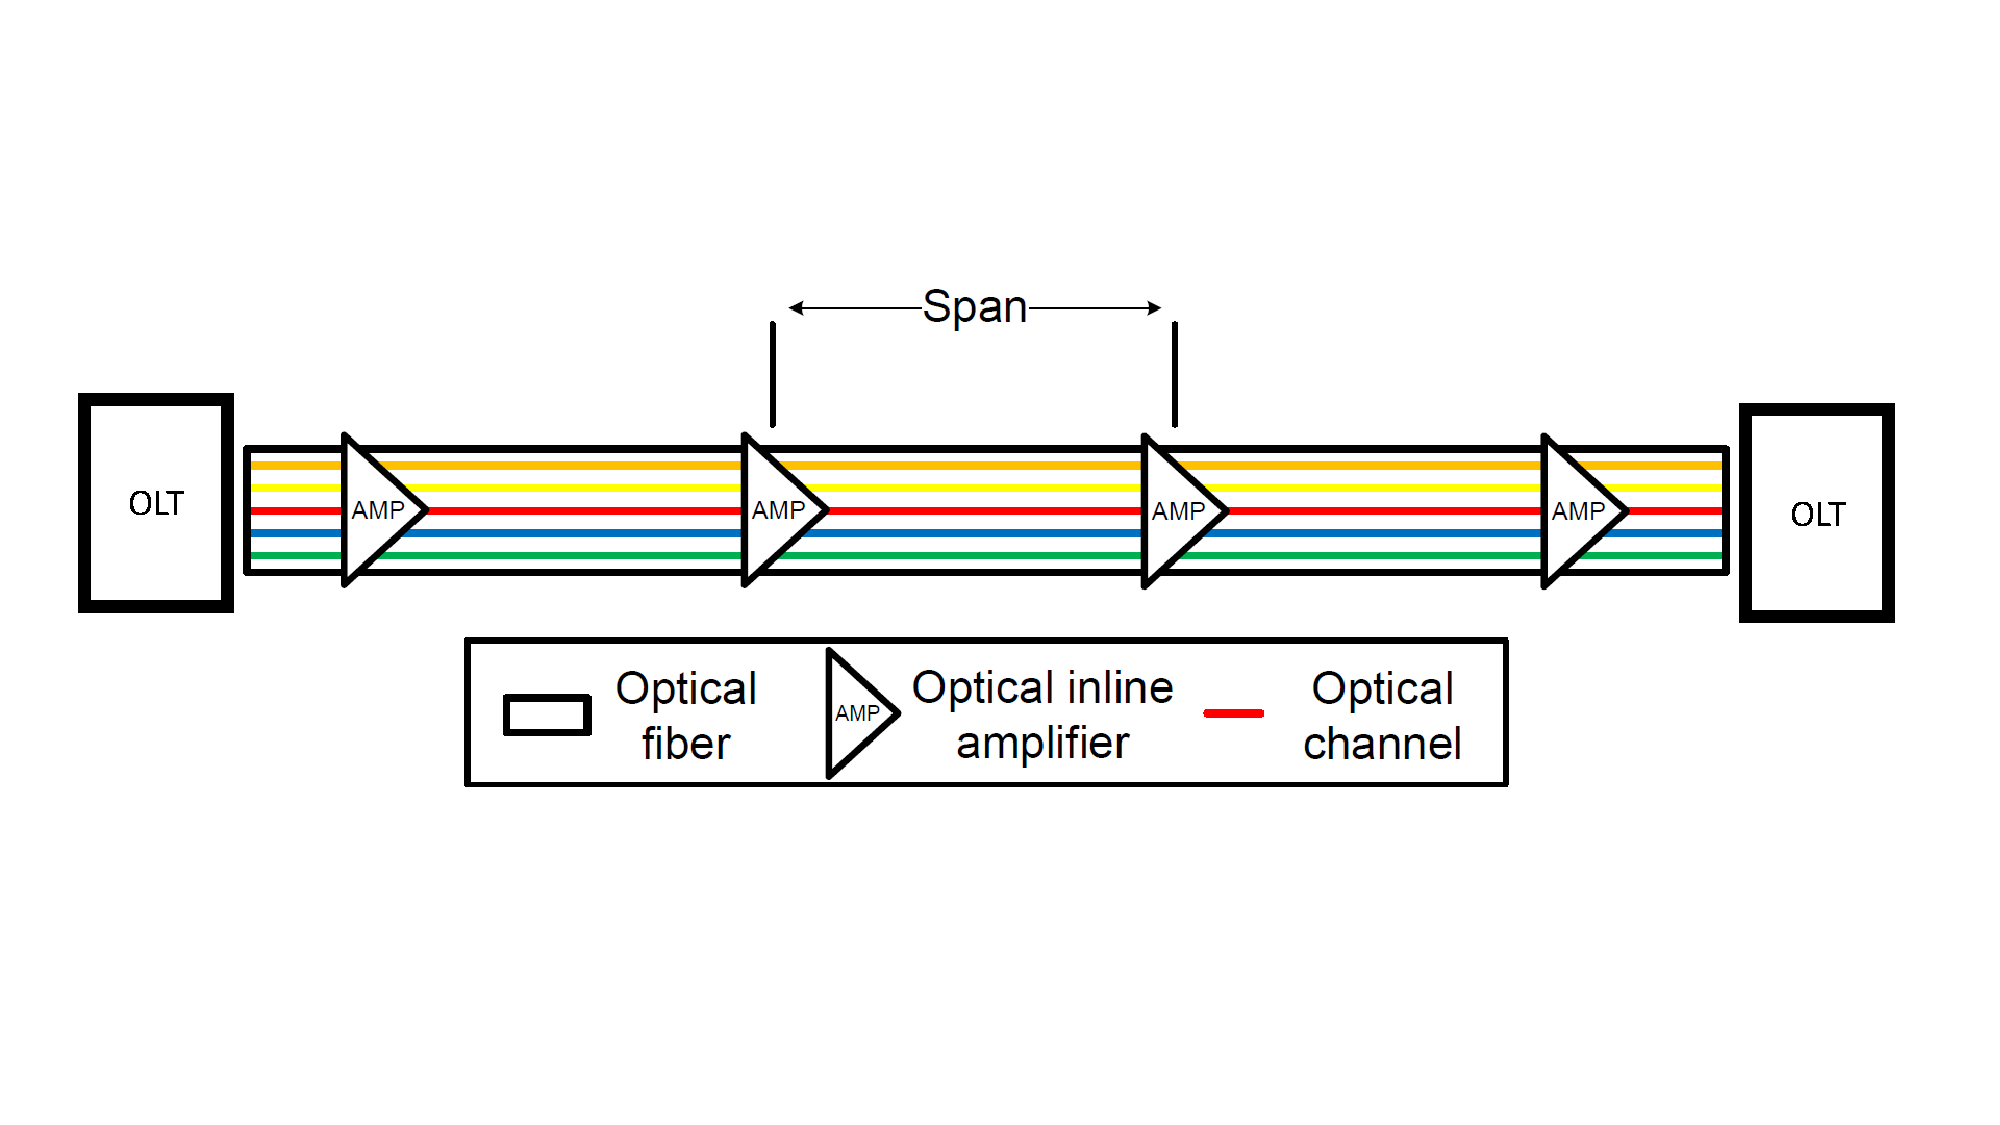
\includegraphics[width=0.7\textwidth]{fig/logos/link.pdf}
    %\caption{Schematic of a link containing an optical fiber, inline optical amplifiers and OLT terminals \cite{RuiMoraisPhD}.}
  \end{center}
\end{figure}

\subsection{Arquitetura dos Nós}

 \begin{figure}[H]
  \label{cisco}
  \begin{center}
    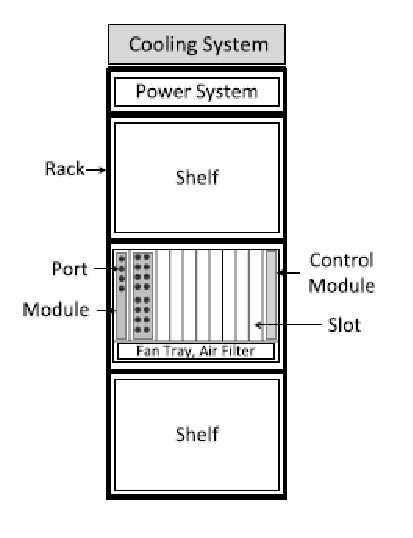
\includegraphics[width=0.40\textwidth]{fig/logos/node.pdf}
    \caption{Schematic of a node structure containing modules, shelves and a rack. \cite{6515886}.}
  \end{center}
\end{figure}

\clearpage

\section{Topologias de Rede}
\label{networkTopologies}
% 1.7 Network Design and Planning ---> Jane Simmons

\subsection{Topologia Física}

\subsection{Topologia Lógica}


\section{Modos de Transporte }
\label{modoTransporte}

\subsection{Modo de Transporte Opaco}
\label{modoTransporteOpaco}

\subsection{Modo de Transporte Transparente}
\label{modoTransporteTransparente}

\section{Rede Referência}
\label{referenceNetwork}

\subsection{Topologia Física}

\begin{figure}[H]
  \begin{center}
    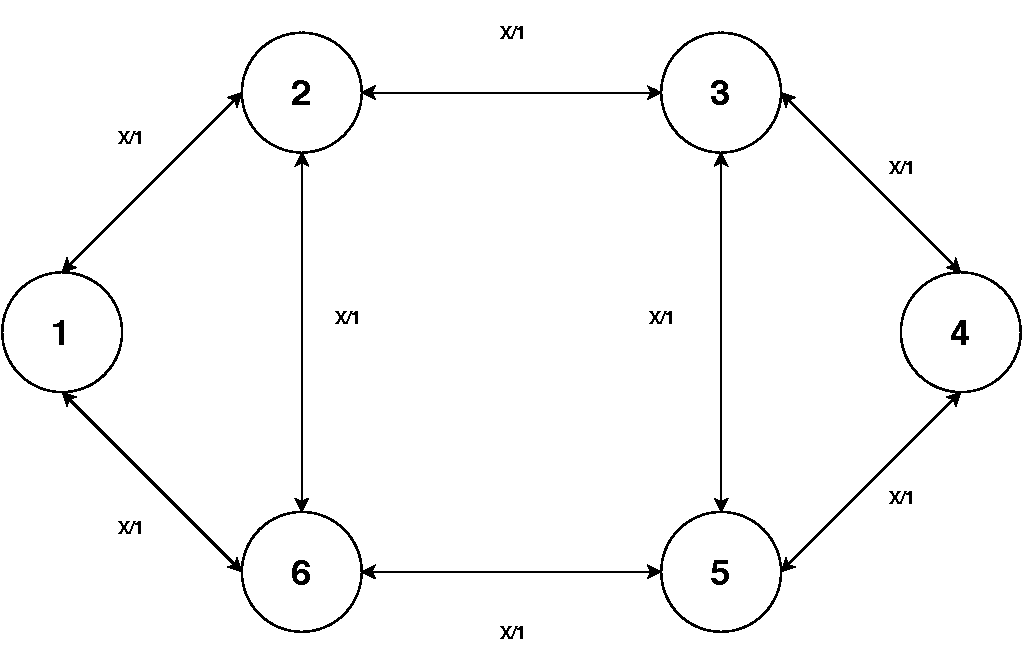
\includegraphics[width=0.7\textwidth]{fig/logos/physicalTopology.pdf}
    \caption{Topologia física da rede referência.}
  \end{center}
   \label{referencePhysical}
\end{figure}

\begin{table}[H]
\centering
\begin{tabular}{|c|c|c|c|c|c|c|}
\hline
\textbf{Node} & \textbf{1} & \textbf{2} & \textbf{3} & \textbf{4} & \textbf{5} & \textbf{6} \\ \hline
\textbf{1} & 0 & 1 & 0 & 0 & 0 & 1 \\ \hline
\textbf{2} & 1 & 0 & 1 & 0 & 0 & 1 \\ \hline
\textbf{3} & 0 & 1 & 0 & 1 & 1 & 0 \\ \hline
\textbf{4} & 0 & 0 & 1 & 0 & 1 & 0 \\ \hline
\textbf{5} & 0 & 0 & 1 & 1 & 0 & 1 \\ \hline
\textbf{6} & 1 & 1 & 0 & 0 & 1 & 0 \\ \hline
\end{tabular}
\caption{Matriz adjacência da topologia física da rede referência.}
\label{referenceAdjacency}
\end{table}
.  
\[
Dist=
  \begin{bmatrix}
    0 & 350 & 0 & 0 & 0 & 150 \\
    350 & 0 & 400 & 0 & 0 & 120 \\
    0 & 400 & 0 & 250 & 100 & 0 \\
    0 & 0 & 250 & 0 & 200 & 0 \\
    0 & 0 & 100 & 200 & 0 & 600 \\
    150 & 120 & 0 & 0 & 600 & 0
  \end{bmatrix}
\]

\subsection{Topologia Lógica}


\subsection{Matrizes de Tráfego}

\subsubsection{Tráfego Baixo}
\label{low}

\[
ODU0=
  \begin{bmatrix}
    0 & 10 & 2 & 6 & 2 & 6 \\
    10 & 0 & 0 & 2 & 10 & 0 \\
    2 & 0 & 0 & 2 & 8 & 2 \\
    6 & 2 & 2 & 0 & 2 & 2 \\
    2 & 10 & 8 & 2 & 0 & 6 \\
    6 & 0 & 2 & 2 & 6 & 0
  \end{bmatrix}
\qquad ODU1=
  \begin{bmatrix}
    0 & 4 & 8 & 4 & 0 & 10 \\
    4 & 0 & 0 & 6 & 2 & 2 \\
    8 & 0 & 0 & 2 & 2 & 0 \\
    4 & 6 & 2 & 0 & 2 & 6 \\
    0 & 2 & 2 & 2 & 0 & 2 \\
    10 & 2 & 0 & 6 & 2 & 0
  \end{bmatrix}
\]
\[
ODU2=
  \begin{bmatrix}
    0 & 2 & 2 & 2 & 0 & 0 \\
    2 & 0 & 0 & 0 & 2 & 0 \\
    2 & 0 & 0 & 2 & 2 & 0 \\
    2 & 0 & 2 & 0 & 2 & 0 \\
    0 & 2 & 2 & 2 & 0 & 2 \\
    0 & 0 & 0 & 0 & 2 & 0
  \end{bmatrix}
\qquad ODU3=
  \begin{bmatrix}
    0 & 0 & 0 & 0 & 0 & 0 \\
    0 & 0 & 2 & 0 & 0 & 2 \\
    0 & 2 & 0 & 0 & 2 & 0 \\
    0 & 0 & 0 & 0 & 0 & 0 \\
    0 & 0 & 2 & 0 & 0 & 0 \\
    0 & 2 & 0 & 0 & 0 & 0
  \end{bmatrix}
\]
\[
ODU4=
  \begin{bmatrix}
    0 & 0 & 0 & 0 & 0 & 0 \\
    0 & 0 & 0 & 0 & 0 & 2 \\
    0 & 0 & 0 & 0 & 0 & 0 \\
    0 & 0 & 0 & 0 & 0 & 0 \\
    0 & 0 & 0 & 0 & 0 & 2 \\
    0 & 2 & 0 & 0 & 2 & 0
  \end{bmatrix}
\]

$T_1^0$ = 120x1.25 = 150 Gbits/s \  $T_1^1$ = 100x2.5 = 250 Gbits/s \  $T_1^2$ = 32x10 = 320 Gbits/s \\

$T_1^3$ = 12x40 = 480 Gbits/s \quad
$T_1^4$ = 8x100 = 800 Gbits/s \\

$T_{1}$ = 150 + 250 + 320 + 480 + 800 = 2000 Gbits/s \qquad
$T$ = 1000/2 = \textbf{1 Tbits/s}\\

\subsubsection{Tráfego Médio}
\label{medium}


\[
ODU0=
  \begin{bmatrix}
    0 & 50 & 10 & 30 & 10 & 30 \\
    50 & 0 & 0 & 10 & 50 & 0 \\
    10 & 0 & 0 & 10 & 40 & 10 \\
    30 & 10 & 10 & 0 & 10 & 10 \\
    10 & 50 & 40 & 10 & 0 & 30 \\
    30 & 0 & 10 & 10 & 30 & 0
  \end{bmatrix}
\quad ODU1=
  \begin{bmatrix}
    0 & 20 & 40 & 20 & 0 & 50 \\
    20 & 0 & 0 & 30 & 10 & 10 \\
    40 & 0 & 0 & 10 & 10 & 0 \\
    20 & 30 & 10 & 0 & 10 & 30 \\
    0 & 10 & 10 & 10 & 0 & 10 \\
    50 & 10 & 0 & 30 & 10 & 0
  \end{bmatrix}
\]
\[
ODU2=
  \begin{bmatrix}
    0 & 10 & 10 & 10 & 0 & 0 \\
    10 & 0 & 0 & 0 & 10 & 0 \\
    10 & 0 & 0 & 10 & 10 & 0 \\
    10 & 0 & 10 & 0 & 10 & 0 \\
    0 & 10 & 10 & 10 & 0 & 10 \\
    0 & 0 & 0 & 0 & 10 & 0
  \end{bmatrix}
\quad ODU3=
  \begin{bmatrix}
    0 & 0 & 0 & 0 & 0 & 0 \\
    0 & 0 & 10 & 0 & 0 & 10 \\
    0 & 10 & 0 & 0 & 10 & 0 \\
    0 & 0 & 0 & 0 & 0 & 0 \\
    0 & 0 & 10 & 0 & 0 & 0 \\
    0 & 10 & 0 & 0 & 0 & 0
  \end{bmatrix}
\]
\[
ODU4=
  \begin{bmatrix}
    0 & 0 & 0 & 0 & 0 & 0 \\
    0 & 0 & 0 & 0 & 0 & 10 \\
    0 & 0 & 0 & 0 & 0 & 0 \\
    0 & 0 & 0 & 0 & 0 & 0 \\
    0 & 0 & 0 & 0 & 0 & 10 \\
    0 & 10 & 0 & 0 & 10 & 0
  \end{bmatrix}
\]


\vspace{17pt}


$T_1^0$ = 600x1.25 = 750 Gbits/s \  $T_1^1$ = 500x2.5 = 1205 Gbits/s \  $T_1^2$ = 160x10 = 1600 Gbits/s \\

$T_1^3$ = 60x40 = 2400 Gbits/s \quad
$T_1^4$ = 40x100 = 4000 Gbits/s \\

$T_{1}$ = 750 + 1250 + 1600 + 2400 + 4000 = 10000 Gbits/s \qquad
$T$ = 10000/2 = \textbf{5 Tbits/s}\\



\subsubsection{Tráfego Elevado}
\label{high}

\[
ODU0=
  \begin{bmatrix}
    0 & 100 & 20 & 60 & 20 & 60 \\
    100 & 0 & 0 & 20 & 100 & 0 \\
    20 & 0 & 0 & 20 & 80 & 20 \\
    60 & 20 & 20 & 0 & 20 & 20 \\
    20 & 100 & 80 & 20 & 0 & 60 \\
    60 & 0 & 20 & 20 & 60 & 0
  \end{bmatrix}
\quad ODU1=
  \begin{bmatrix}
    0 & 40 & 80 & 40 & 0 & 100 \\
    40 & 0 & 0 & 60 & 20 & 20 \\
    80 & 0 & 0 & 20 & 20 & 0 \\
    40 & 60 & 20 & 0 & 20 & 60 \\
    0 & 20 & 20 & 20 & 0 & 20 \\
    100 & 20 & 0 & 60 & 20 & 0
  \end{bmatrix}
\]
\[
ODU2=
  \begin{bmatrix}
    0 & 20 & 20 & 20 & 0 & 0 \\
    20 & 0 & 0 & 0 & 20 & 0 \\
    20 & 0 & 0 & 20 & 20 & 0 \\
    20 & 0 & 20 & 0 & 20 & 0 \\
    0 & 20 & 20 & 20 & 0 & 20 \\
    0 & 0 & 0 & 0 & 20 & 0
  \end{bmatrix}
\quad ODU3=
  \begin{bmatrix}
    0 & 0 & 0 & 0 & 0 & 0 \\
    0 & 0 & 20 & 0 & 0 & 20 \\
    0 & 20 & 0 & 0 & 20 & 0 \\
    0 & 0 & 0 & 0 & 0 & 0 \\
    0 & 0 & 20 & 0 & 0 & 0 \\
    0 & 20 & 0 & 0 & 0 & 0
  \end{bmatrix}
\]
\[
ODU4=
  \begin{bmatrix}
    0 & 0 & 0 & 0 & 0 & 0 \\
    0 & 0 & 0 & 0 & 0 & 20 \\
    0 & 0 & 0 & 0 & 0 & 0 \\
    0 & 0 & 0 & 0 & 0 & 0 \\
    0 & 0 & 0 & 0 & 0 & 20 \\
    0 & 20 & 0 & 0 & 20 & 0
  \end{bmatrix}
\]

\vspace{17pt}

$T_1^0$ = 1200x1.25 = 1500 Gbits/s \qquad
$T_1^1$ = 1000x2.5 = 2500 Gbits/s \\

$T_1^2$ = 320x10 = 3200 Gbits/s \qquad
$T_1^3$ = 120x40 = 4800 Gbits/s \\

$T_1^4$ = 80x100 = 8000 Gbits/s \qquad
$T_{1}$ = 20000 Gbits/s \\

$T$ = 20000/2 = \textbf{10 Tbits/s}

\section{Rede Real}
\label{realisticNetwork}


\subsection{Topologia Física}


\subsection{Matrizes de Tráfego}
\label{referenceTraffic}




\cleardoublepage